\documentclass[tikz,border=3pt]{standalone}
\usepackage[utf8]{inputenc}
\usepackage[T1]{fontenc}
\usepackage{lmodern}
\renewcommand{\familydefault}{\sfdefault}
\usepackage{sansmath}\sansmath
\usepackage{chemfig}
\usepackage{pgfplots}\pgfplotsset{compat=1.18,/pgf/number format/use comma,/pgf/number format/1000 sep={.}}
\usetikzlibrary{arrows.meta,calc,positioning,decorations.pathmorphing,patterns}
% paleta del sitio
\definecolor{nar}{HTML}{E8680C}\definecolor{narc}{HTML}{FFB35C}\definecolor{hielo}{HTML}{FFF3E8}
\definecolor{tinta}{HTML}{1D1D1F}\definecolor{gris}{HTML}{6E6E73}\definecolor{lila}{HTML}{7C5CF0}
\definecolor{azul}{HTML}{2F6FD6}\definecolor{menta}{HTML}{17A673}\definecolor{coral}{HTML}{E8342A}
\begin{document}
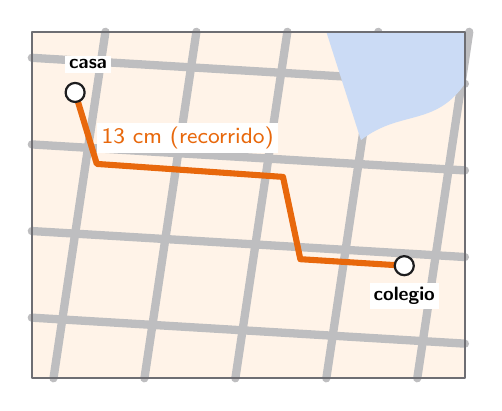
\begin{tikzpicture}[font=\small,x=0.55cm,y=0.55cm,line cap=round,line join=round,step={(1,1)}]
\fill[hielo] (0,0) rectangle (10,8);
\draw[gris!45,line width=3pt] (0.5,0)--(1.7,8);
\draw[gris!45,line width=3pt] (2.6,0)--(3.8,8);
\draw[gris!45,line width=3pt] (4.7,0)--(5.9,8);
\draw[gris!45,line width=3pt] (6.8,0)--(8.0,8);
\draw[gris!45,line width=3pt] (8.9,0)--(10.1,8);
\draw[gris!45,line width=3pt] (0,1.4)--(10,0.7999999999999999);
\draw[gris!45,line width=3pt] (0,3.4)--(10,2.8);
\draw[gris!45,line width=3pt] (0,5.4)--(10,4.800000000000001);
\draw[gris!45,line width=3pt] (0,7.4)--(10,6.800000000000001);
\fill[azul!25] (7.6,5.5) .. controls (8.5,6.2) and (9.3,5.8) .. (10,6.8)--(10,8)--(6.8,8)--cycle;
\draw[gris,thick] (0,0) rectangle (10,8);
\draw[nar,line width=2.2pt] (1.0,6.6)--(1.5,4.95)--(5.8,4.65)--(6.2,2.75)--(8.6,2.6);
\filldraw[fill=white,draw=tinta,thick] (1.0,6.6) circle (0.22); \filldraw[fill=white,draw=tinta,thick] (8.6,2.6) circle (0.22);
\node[font=\scriptsize\bfseries,fill=white,inner sep=1.5pt] at (1.3,7.25) {casa};
\node[font=\scriptsize\bfseries,fill=white,inner sep=1.5pt] at (8.6,1.9) {colegio};
\node[font=\footnotesize,fill=white,inner sep=1.5pt,text=nar] at (3.6,5.55) {13 cm (recorrido)};
\end{tikzpicture}
\end{document}
